\section{Data}%
\label{sec:Data}%
This is what some of the data looks like.It is a \href{https://scikit-learn.org/stable/datasets/index.html#diabetes-dataset}{dataset on diabetes}.
The data originated from a \href{https://www4.stat.ncsu.edu/~boos/var.select/diabetes.html}{LARS Paper}.
\newline
There are 442 instances with 10 baseline variables. The response of interest 
is a quantitative measure of disease progression one year after baseline.
\newline
Each of these 10 feature variables have been mean centered and scaled 
by the standard deviation times n\_samples 
(i.e. the sum of squares of each column totals 1).\\ 
\[\frac{x-\mu}{\sigma}\]

\begin{center}\begin{tabular}{lrrrrrrrrrr}
\toprule
{} &    age &    sex &    bmi &     bp &     s1 &     s2 &     s3 &     s4 &     s5 &     s6 \\
\midrule
count & 442.00 & 442.00 & 442.00 & 442.00 & 442.00 & 442.00 & 442.00 & 442.00 & 442.00 & 442.00 \\
mean  &  -0.00 &   0.00 &  -0.00 &   0.00 &  -0.00 &   0.00 &  -0.00 &   0.00 &  -0.00 &  -0.00 \\
std   &   0.05 &   0.05 &   0.05 &   0.05 &   0.05 &   0.05 &   0.05 &   0.05 &   0.05 &   0.05 \\
min   &  -0.11 &  -0.04 &  -0.09 &  -0.11 &  -0.13 &  -0.12 &  -0.10 &  -0.08 &  -0.13 &  -0.14 \\
25\%   &  -0.04 &  -0.04 &  -0.03 &  -0.04 &  -0.03 &  -0.03 &  -0.04 &  -0.04 &  -0.03 &  -0.03 \\
50\%   &   0.01 &  -0.04 &  -0.01 &  -0.01 &  -0.00 &  -0.00 &  -0.01 &  -0.00 &  -0.00 &  -0.00 \\
75\%   &   0.04 &   0.05 &   0.03 &   0.04 &   0.03 &   0.03 &   0.03 &   0.03 &   0.03 &   0.03 \\
max   &   0.11 &   0.05 &   0.17 &   0.13 &   0.15 &   0.20 &   0.18 &   0.19 &   0.13 &   0.14 \\
\bottomrule
\end{tabular}\end{center}
\\\centerline{\caption{Descriptive table of diabetes data.}}%

\begin{figure}[!ht]%
\centering%
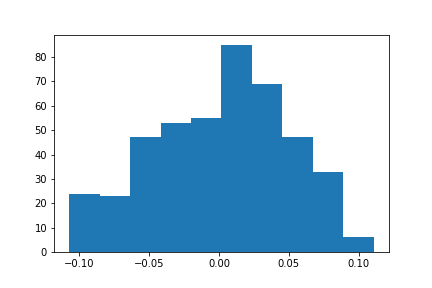
\includegraphics[width=0.75\textwidth]{../figures/Figure2.png}%
\linebreak%
\caption{This image was saved directly to the current folder.}%
\end{figure}
\\
\lipsum[3-4]

\subsection{By the Way}
\label{subsec:byTheWay}
If you would like to merge multiple dataframes together, you can just pass them in
as a list of tables to be added. The output will be something like:
\begin{tabular}{lrrr}
\toprule
{} &     s1 &     s3 &     s5 \\
\midrule
count & 442.00 & 442.00 & 442.00 \\
mean  &  -0.00 &  -0.00 &  -0.00 \\
std   &   0.05 &   0.05 &   0.05 \\
min   &  -0.13 &  -0.10 &  -0.13 \\
25\%   &  -0.03 &  -0.04 &  -0.03 \\
50\%   &  -0.00 &  -0.01 &  -0.00 \\
75\%   &   0.03 &   0.03 &   0.03 \\
max   &   0.15 &   0.18 &   0.13 \\
\bottomrule
\end{tabular}
\\\caption{Merged dataframes example.}
